\definecolor{acmBlue}{HTML}{1F77B4}
\definecolor{acmTeal}{HTML}{009E73}
\definecolor{acmSand}{HTML}{D55E00}
\definecolor{acmGrid}{HTML}{D9DDE2}
\definecolor{acmGray}{HTML}{8A8F99}
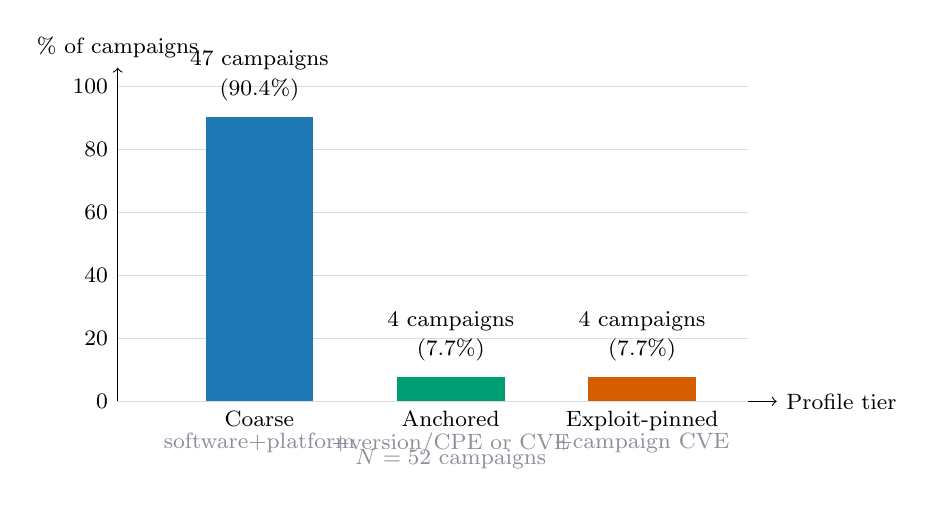
\begin{tikzpicture}[x=1.80cm,y=0.040cm,font=\footnotesize]
  \draw[->] (0,0) -- (4.65,0) node[right] {Profile tier};
  \draw[->] (0,0) -- (0,106) node[above] {\% of campaigns};
  \foreach \yy in {0,20,40,60,80,100} {
    \draw[acmGrid] (0,\yy) -- (4.45,\yy);
    \node[left] at (0,\yy) {\yy};
  }

  \fill[acmBlue] (0.62,0) rectangle (1.38,90.4);
  \fill[acmTeal] (1.97,0) rectangle (2.73,7.7);
  \fill[acmSand] (3.32,0) rectangle (4.08,7.7);

  \node[below] at (1.00,0) {Coarse};
  \node[below] at (2.35,0) {Anchored};
  \node[below] at (3.70,0) {Exploit-pinned};

  \node[below,font=\footnotesize,text=acmGray] at (1.00,-7.0) {software+platform};
  \node[below,font=\footnotesize,text=acmGray] at (2.35,-7.0) {+version/CPE or CVE};
  \node[below,font=\footnotesize,text=acmGray] at (3.70,-7.0) {+campaign CVE};

  \node[above,align=center] at (1.00,92.4) {\shortstack{47 campaigns\\(90.4\%)}};
  \node[above,align=center] at (2.35,9.7) {\shortstack{4 campaigns\\(7.7\%)}};
  \node[above,align=center] at (3.70,9.7) {\shortstack{4 campaigns\\(7.7\%)}};

  \node[below,font=\footnotesize,text=acmGray] at (2.35,-12.0) {$N=52$ campaigns};
\end{tikzpicture}
